\chapter{Planificación y Metodología}
\label{chap:metodos}
En este apartado se discutirán los métodos empleados para el desarrollo del proyecto así como las decisiones tomadas a lo largo del mismo que llevaron al uso y configuración de estos.


\section{Software}
\subsection{Entorno de desarrollo}
\lettrine{T}{odo} el proyecto se llevó a cabo como parte del trabajo previo de \citeauthor{IglesiasGuitian2022}. Esto trae consigo una serie de restricciones con respecto al software utilizado. Con el fin de minimizar las dependencias y los errores a la hora de la integración, se desarrolló en C++, en el \acrshort{ide} Visual Studio 2022. Como sistema operativo se utilizó Windows, replicando el proyecto raíz.
\subsection{Impresión 3D}
Para el proceso de la impresión del modelo anatomico se tomó como referencia el protocolo definido en \citeauthor{MoretaMartinez2020} que hace uso de 3DSlicer (https://www.slicer.org/) para seleccionar que partes del modelo anatómico deseamos utilizar como referencia en el mundo real, en caso de querer utilizar alguna. Se utilizó una impresora Ultimaker 3 de doble cabezal.

Con el fin de disipar cualquier tipo de error producto del desarrollo, se trabajó con un único \acrshort{tc}. Una vez cargado en 3DSlicer se nos presenta una pantalla similar a \ref{fig:cap3DSlicer}. 
Mediante las herramientas de selección de volúmenes que se ven en \ref{fig:segmentEditor} se creó un volumen que posteriormente, con el fin de obtener un objeto completo imprimible, se corrigió respetando las formas originales usando Meshmixer.
Dada la complejidad de la pieza, se hizo uso de la impresora de polvo de vinilo que se encuentra en el \acrshort{citic}, dando lugar a la pieza que se ve en \ref{fig:craneoVinilo}.



\begin{figure}[hp!]
  \centering
  \includegraphics[width=0.75\textwidth]{imaxes/captura_3DSlicer.png}
  \caption{Captura de pantalla de 3DSlicer.}
  \label{fig:cap3DSlicer}
\end{figure}
\begin{figure}[hp!]
  \centering
  \includegraphics[width=0.75\textwidth]{imaxes/segment_editor.png}
  \caption{Captura de pantalla de las herramientas de selección de segmentos.}
  \label{fig:segmentEditor}
\end{figure}
\begin{figure}[hp!]
  \centering
  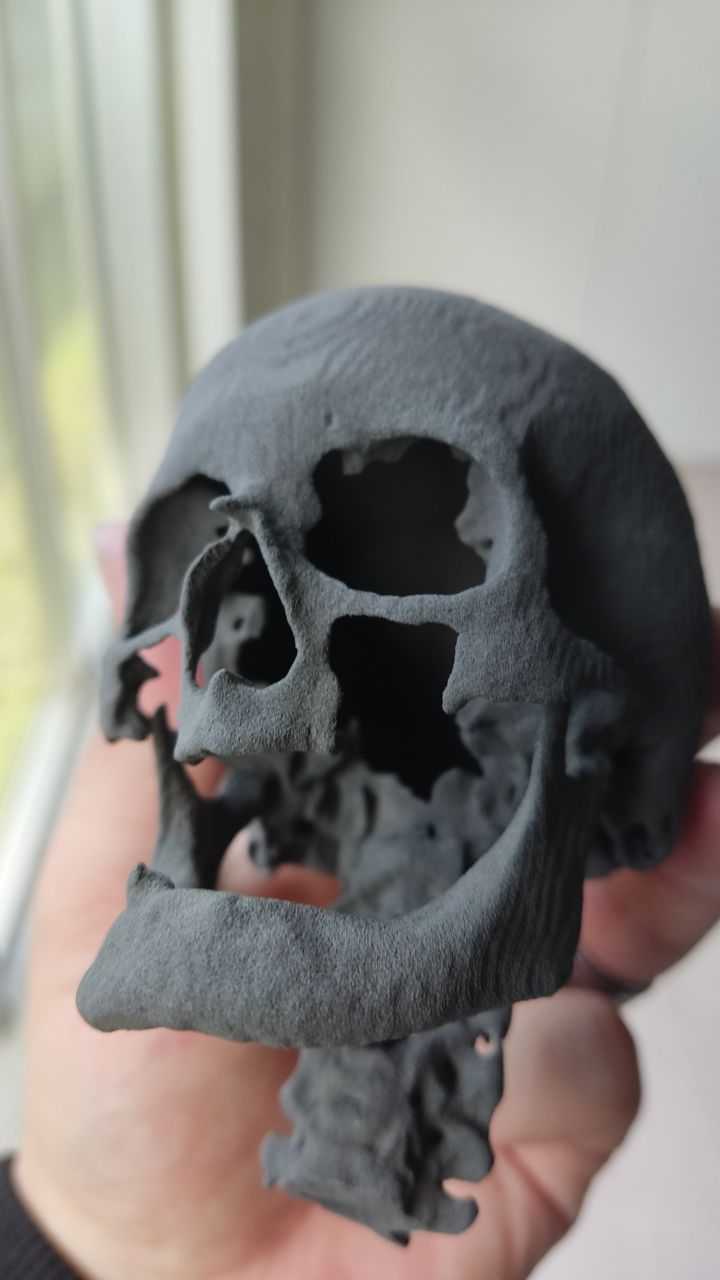
\includegraphics[width=0.75\textwidth]{imaxes/craneo_vinilo.jpg}
  \caption{Pieza impresa en polvo de vinilo}
  \label{fig:craneoVinilo}
\end{figure} 
\subsection{Tracking}
Debido a la complejidad que puede alcanzar implementar desde cero un algoritmo de seguimiento, se utilizo la librería OpenCV (https://opencv.org/) para llevar a cabo tanto el diseño del marcador como el seguimiento del mismo.

\subsection{Visualización}
Se utilizó el \acrshort{hmd} HTC Vive Pro para probar la parte relacionada con el visionado de la 
